\section{Evaluation}
% The experimental results are presented and analyzed in this section.
% In detail, experimental settings are introduced in Sec.~\ref{sec:experiment-settings}.
% Sec.~\ref{sec:experiment-e2e}-Sec.~\ref{sec:experiment-case-study} conduct the end-end experiments, test on queries with cycles, perform ablation studies, evaluate the optimization efficiency, test the efficiency of optimziations accross reltaional and graph queries, and evaluate the efficiency of the join order of the plans generated by \relgo, respectively.

\begin{table}[t]
    \centering
    \begin{tabular}{c|c|c|c}
    \hline
    Dataset & |V| & |E| & Disk Space Usage\\ 
    \hline
    $G_{sf10}$& 29,987,835 & 88,317,856 & 8.9G \\
    \hline
    $G_{sf30}$ & 88,789,833 & 278,652,443 & 28.0G\\
    \hline
    $IMDB$ & 14,431,946 & 59,758,241 & 3.7G \\
    \hline
    \end{tabular}
    \caption{Statistics of the datasets. In detail, $|\cdot|$ represents the number of elements in $\cdot$.}
    \label{table:experiment-datasets}
\end{table}

\subsection{Experimental Settings}
\label{sec:experiment-settings}
\noindent\textbf{Compared Systems. }
We compare \relgo against two state-of-art baseline systems: DuckDB~\cite{duckdb} as a representative of $Rel$ optimizers, and GrainDB~\cite{graindb} as a representative of $Rel^+$ optimizers.
For fair comparison, we use the backend of DuckDB of version 0.9.2 as the common backend for all compared systems. 
For GrainDB, we first upgraded the integrated DuckDB backend to v0.9.2, and then after the optimized physical plans are obtained, GrainDB's optimizer will further replace some hash joins with sip joins (or merge sip joins), so as to leverage the graph indices.
For \relgo, after the optimized physical plans are obtained, it replace the \todo{extend-intersect operators} with appropriate join implementations, including hash joins, or sip joins (or merge sip joins) according to the graph indices.
Therefore, different plans can be executed on the same backend of DuckDB, and the efficiency of the plans obtained by varied optimizers can be compared fairly.
Note that codegen techniques can be employed to facilitate the transformation of the physical plans.
For simplicity, in the following, when there is no ambiguity, the optimizers of DuckDB and GrainDB are shortened to DuckDB and GrainDB, respectively.

\noindent\textbf{Benchmarks.} In the experiments, two commonly-used benchmarks are leveraged.
\begin{itemize}
    \item \textbf{LDBC SNB.} The Linked Data Benchmark Council (LDBC) Social Network Benchmark~\cite{ldbc_snb} is utilized. We adopted two datasets of $G_{sf10}$ and $G_{sf30}$, generated by LDBC data generator with scale factor 10 and 30 respectively.
    The LDBC Interactive Complex workloads, denoted as  $IC[1, \ldots, 9, 11, 12]$, are used to evaluate the performance of \relgo, with $IC[10]$, $IC[13]$, and $IC[14]$ excluded since they involve either pre-computation or shortest-path that are not supported.
    The queries containing variable-length joins are broken down to several individual queries with a suffix ``$-l$'' denoting the fixed length, as following~\cite{graindb}.
    In addition, we carefully designed two categories of queries for the comprehensiveness of evaluation, including (1) $Q_r[1\ldots 7]$ to test the effectiveness of heuristic rules in \relgo, and (2) $Q_c[1\ldots 3]$, comprising three typical patterns with cycles including triangle, square, and 4-clique, respectively, to evaluate the efficiency of the cost-based optimization techniques in \relgo.
    \item \textbf{JOB.} The Join Order Benchmark (JOB)~\cite{job_snb} on Internet Movie Database (IMDB) is adopted. We select the ``a'' variant of JOB queries, referred to as $JOB[1\ldots 33]$, without loss of generality. These queries are primarily designed to test join order optimization, with each query containing an average of $8$ joins.
\end{itemize}
The details of the dataset statistics are summarized in Table \ref{table:experiment-datasets}, and the queries are listed in \todo{appendix}.
Note that we prepared the datasets for the experiments by constructing indices using the same methodology as described in~\cite{graindb}.
In the experiments, we run each query for \todo{10 times} and report the average execution time cost.
we set the timeout for each query to be \todo{1 hour}, and queries that fail to finish within the timeout are marked as \ot.
Besides, we set the parallelism to be 1 for all the experiments.

The experiments are carried out on a server with Intel Xeon E5-2682 2.50GHz CPU and 251GB RAM.

\subsection{Micro Benchmarks on Graph Optimizers}
\label{sec:experiment-opt}
In this subsection, we conduct micro benchmarks to evaluate the efficiency of the optimization techniques in \relgo.

% \noindent\textbf{Optimization Efficiency Evaluation.}
% In this subsection, experiments are conducted to compare the optimization time cost of \relgo and Apache Calcite, which is a well-known data management framework widely used in various projects such as Hive and Kylin.
% Please note that the codes of \relgo and Calcite are both written in Java.
% In detail, we test the optimization time of \relgo and Calcite on SNB-M and JOB benchmarks, and VolcanoPlanner of Calcite with default rules is leveraged.
% If optimization for a query is not finished in 10 minutes, the process is early stopped and the time cost of such optimization is recorded as 10 minutes.
% The results are shown in Fig.~\ref{fig:exp-optimization}.

% \begin{figure*}[ht]
%     \centering
%     \begin{subfigure}[b]{0.3\linewidth}
%         \centering
%         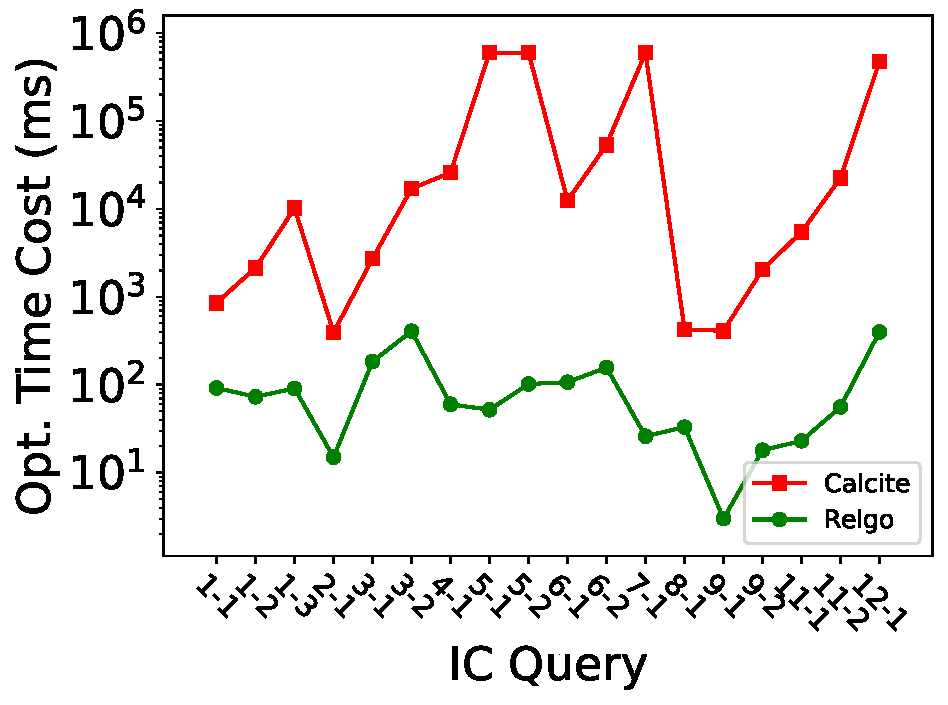
\includegraphics[width=\linewidth]{./figures/exp/optimization_sf10.pdf}
%         \caption{Optimization Time Cost on $G_{sf10}$.}
%         \label{fig:exp-optimization-sf10}
%     \end{subfigure}
%     \begin{subfigure}[b]{0.3\linewidth}
%         \centering
%         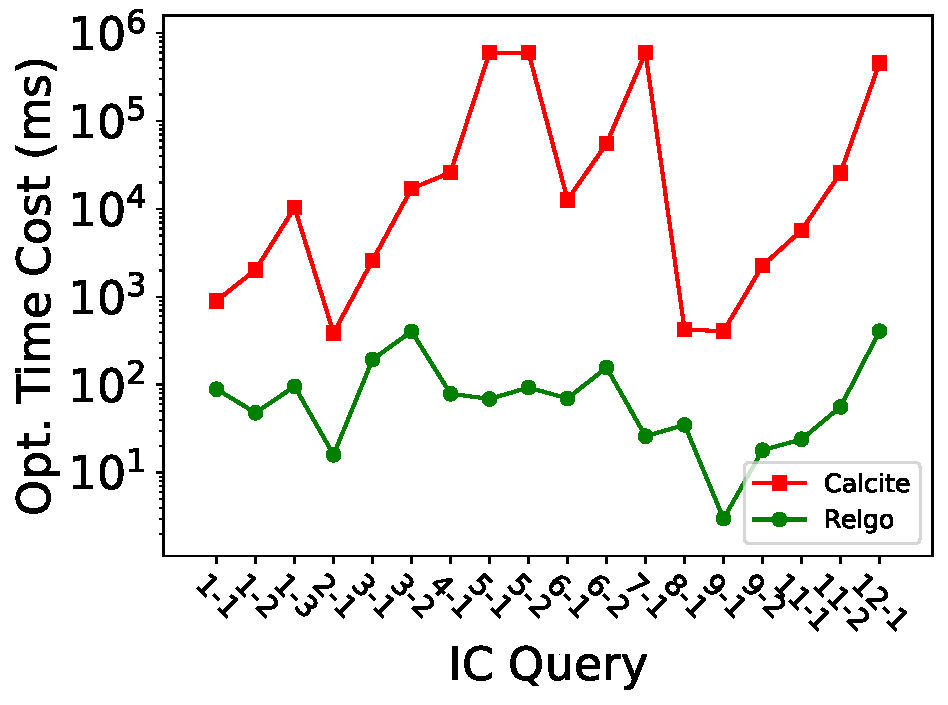
\includegraphics[width=\linewidth]{./figures/exp/optimization_sf30.pdf}
%         \caption{Optimization Time Cost on $G_{sf30}$.}
%         \label{fig:exp-optimization-sf30}
%     \end{subfigure}
%     \begin{subfigure}[b]{0.3\linewidth}
%         \centering
%         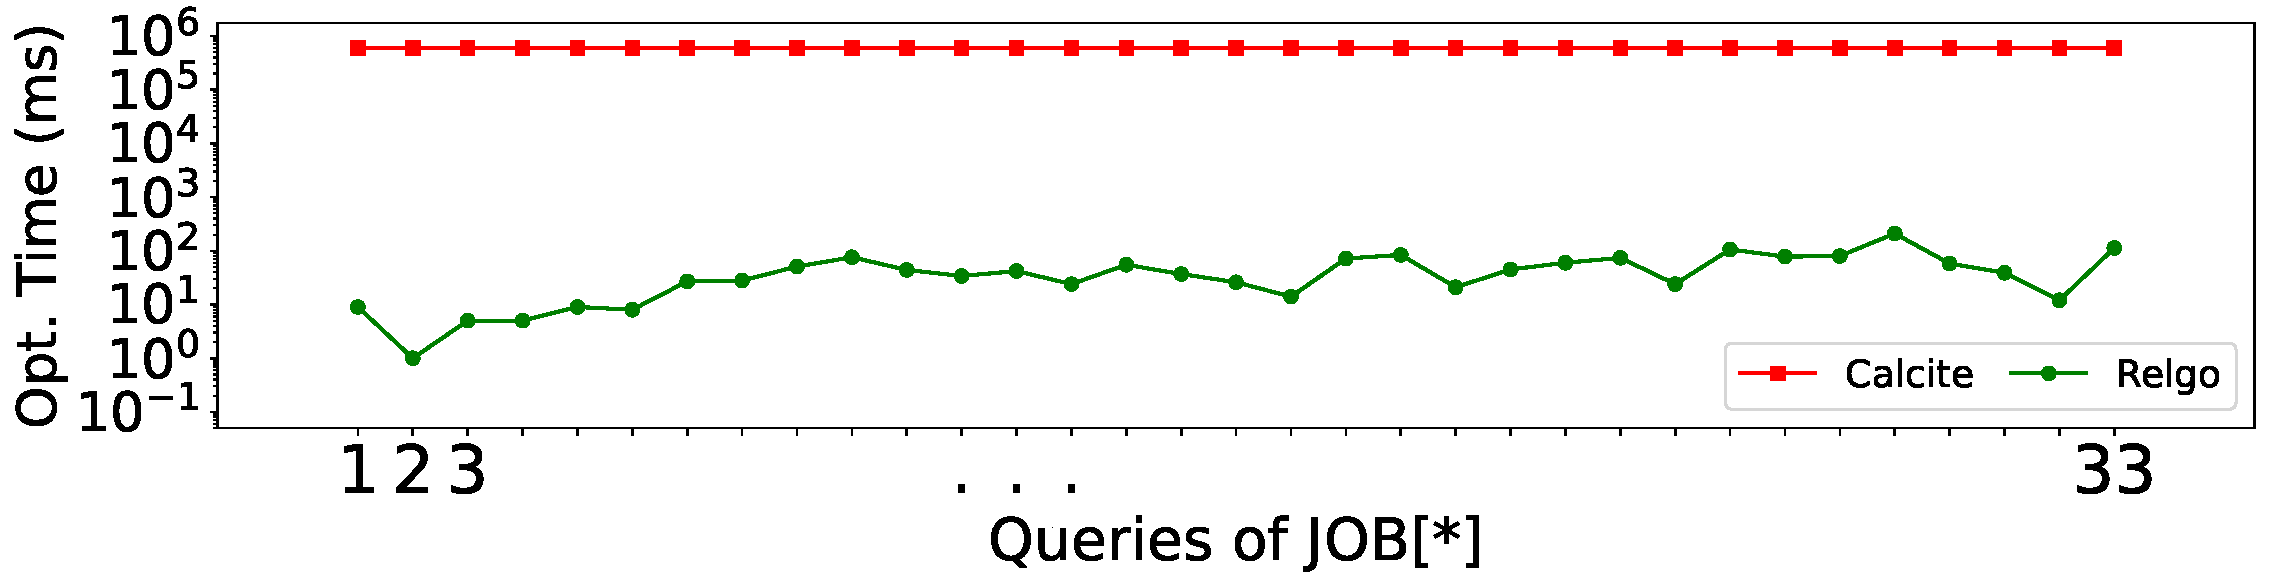
\includegraphics[width=\linewidth]{./figures/exp/optimization_job.pdf}
%         \caption{Optimization Time Cost on IMDB.}
%         \label{fig:exp-optimization-job}
%     \end{subfigure}
%     \caption{Experiments on the time cost of optimization.}
%     \label{fig:exp-optimization}
% \end{figure*}

% In the experiments, optimizing all the queries with \relgo can be finished in 10 minutes, while optimizing some queries with Calcite exceeds the 10-minute limit.
% For example, when JOB benchmark is utilized, the time cost of optimizing all the queries with Calcite is longer than 10 minutes.
% As shown in Fig.~\ref{fig:exp-optimization}, \relgo is much more efficient than Calcite in optimizing queries, and it is consistent with the conclusions obtained in Sec.~\ref{sec:theoretical-analysis}.
% That is, \relgo is exponentially faster than Calcite in query optimization.
% For instance, when IC5-1 is queried on $G_{sf30}$, the time cost of query optimization with \relgo can be more than $10^4\times$ faster than that of Calcite.

% Besides, the optimization time cost of \relgo is similar on $G_{sf10}$ and $G_{sf30}$, and so is Calcite.
% The reason is that the time required for optimization is not significantly associated with the scale of the dataset; instead, it is related to the relative cardinalities among the different tables.
% The relative cardinalities in LDBC datasets of different scales are consistent, therefore the optimization time is similar.

\begin{figure}[ht]
    \centering
    \begin{subfigure}[b]{.45\linewidth}
        \centering
        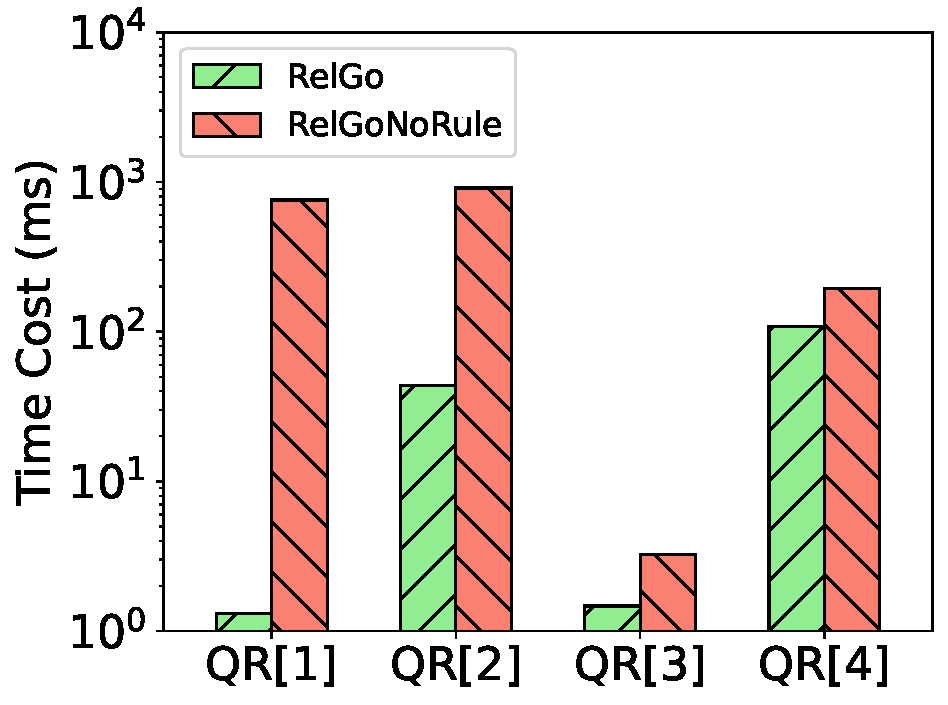
\includegraphics[width=\linewidth]{./figures/exp/filter_sf10.pdf}
        \caption{Time Cost on $G_{sf10}$.}
        \label{fig:exp-filter-sf10}
    \end{subfigure}
    \begin{subfigure}[b]{0.45\linewidth}
        \centering
        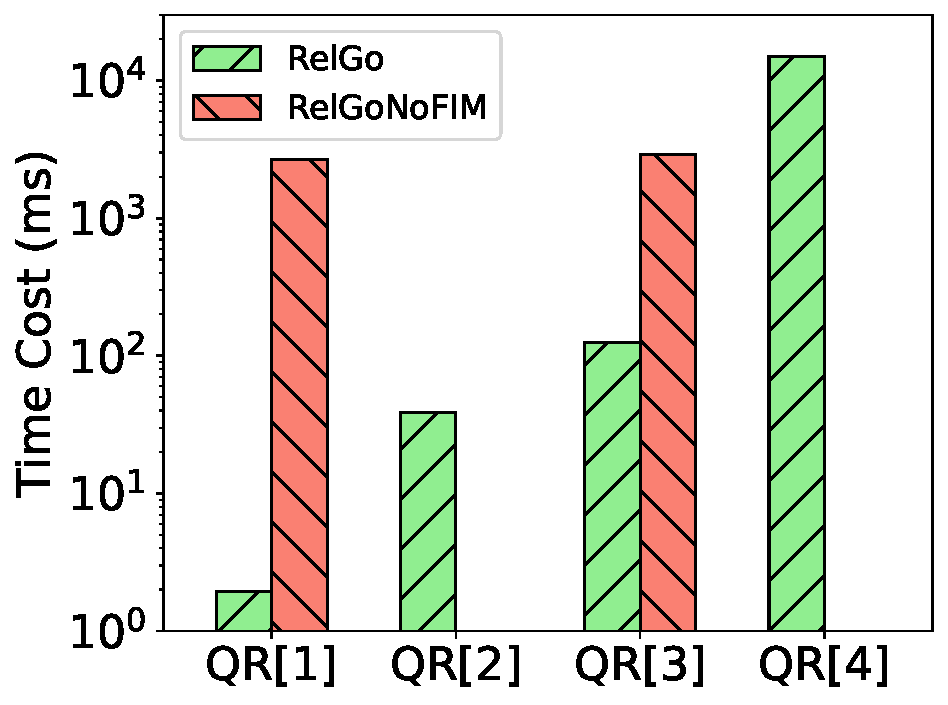
\includegraphics[width=\linewidth]{./figures/exp/filter_sf30.pdf}
        \caption{Time Cost on $G_{sf30}$.}
        \label{fig:exp-filter-sf30}
    \end{subfigure}
    \caption{Comparison of efficiency between \relgo and \textit{\relgo w.o. inter}.}
    \label{fig:exp-filter}
\end{figure}

\noindent\textbf{Rule-based Optimization.}
As highlighted in \todo{Section~\ref{sec:rbo}}, \filterrule is employed in \relgo to capture the optimization opportunities at the interplay of relational and graph queries. \todo{more rules}.
We compare the performance of \relgo with and without (denoted as \relgo w.o.~Inter) \filterrule on $G_{sf10}$ and $G_{sf30}$, and show the results in Fig.~\ref{fig:exp-filter}.
he results suggest that \filterrule~ enhanced the efficiency of \relgo~ by \todo{xx} times on average on $G_{sf10}$, and \todo{xx} times on $G_{sf30}$.
\todo{why no improvement?}
Please note that \relgo and \textit{\relgo w.o.~inter} have similar performances on some queries, e.g., SP6-1 and SP11-1.
The reason is that \filterrule is primarily in effect in these queries.
However, the pruning effect induced by constraints delineated within the relational query portion is comparatively marginal, while the pruning effect of the other constraints within the graph query portion is highly effective.
Consequently, whether to apply \filterrule to push the filter constraints down into graph queries has limited influence in these queries.

\begin{figure}[ht]
    \centering
    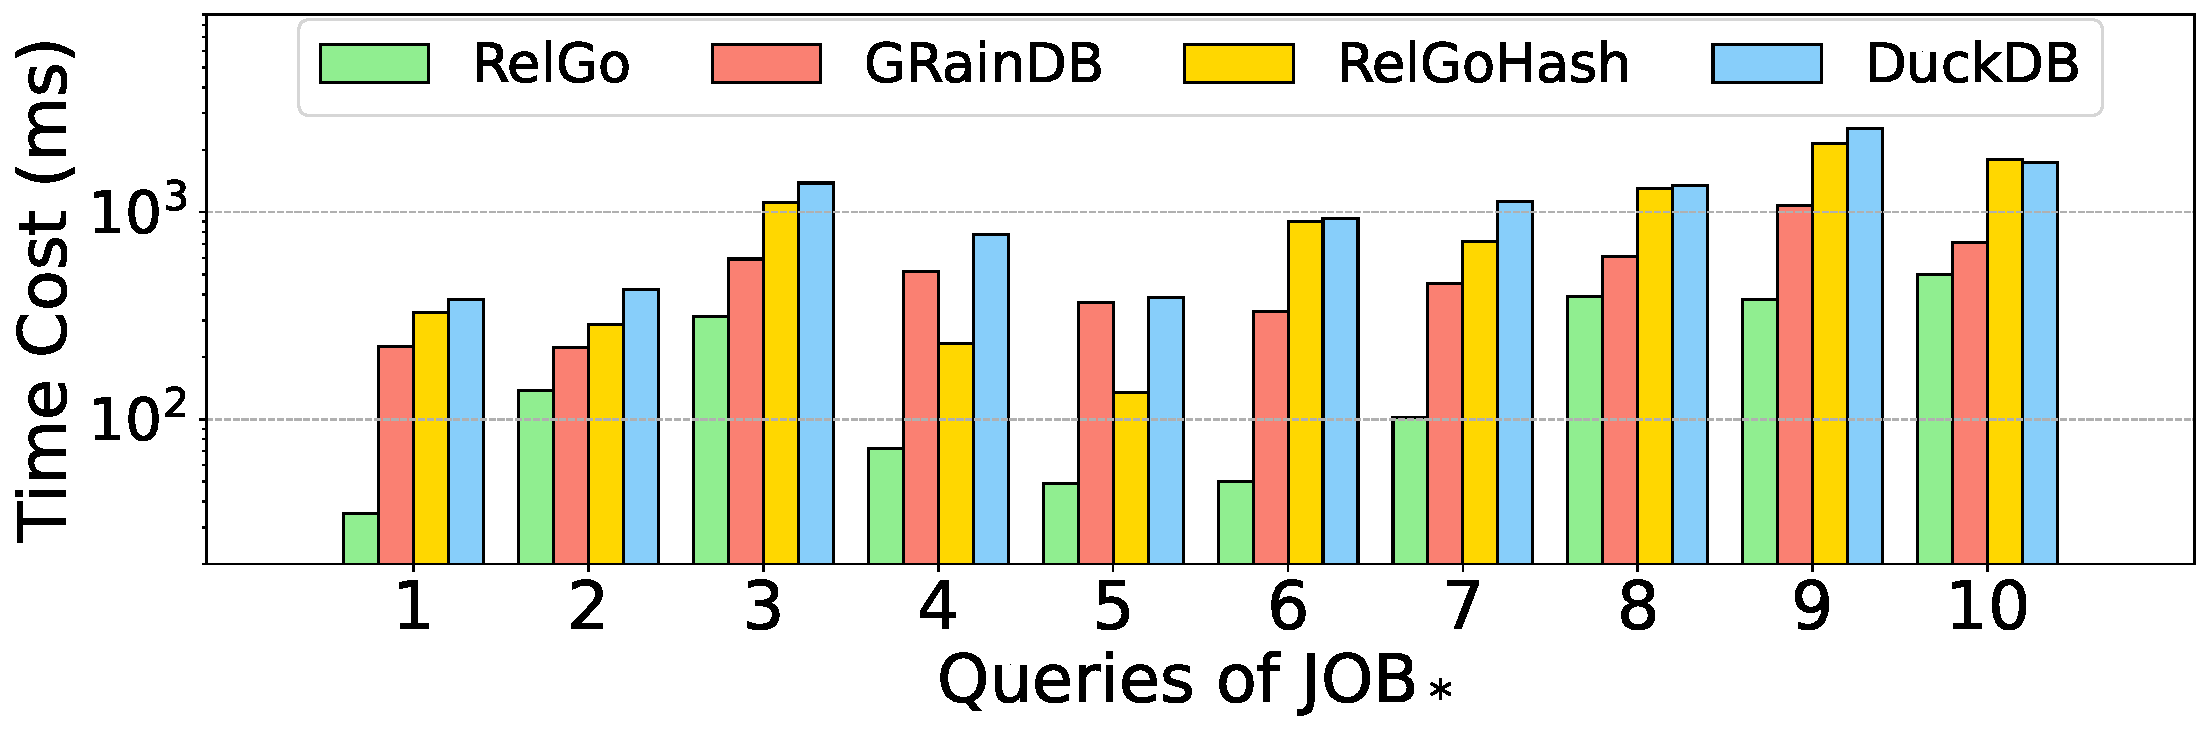
\includegraphics[width=.9\linewidth]{./figures/exp/hash_plan_job.pdf}
    \caption{Experiments that compare the efficiency of \relgo and \relgo-hash.}
    \label{fig:exp-hash-plan}
\end{figure}
\noindent\textbf{Cost-based Optimization.}
Then we assess the effectiveness of the cost-based optimization techniques in \relgo.

First we compare the performance of \relgo with GrainDB and DuckDB on IMDB to evaluate their optimized plans.
In details, in addition to \relgo which replace the extend-intersect operators with different join implementations based on whether the graph indices can be utilized, we further implement a variant of \relgo, named \relgohash, which replaces all the extend-intersect operators with hash joins, indicating that the graph indices are not utilized, so as to obtain a more fair comparison with DuckDB.
Without loss of generality, queries $JOB[1\ldots 10]$ are utilized as the representatives in the experiments.
The performance results are shown in Fig.~\ref{fig:exp-hash-plan}. \todo{separate the figure? since we may not want to highlight that \relgo always output superior join orders, that \relgohash is even better than GrainDB.}
From the results, we can observe that \relgo outperforms GrainDB on all the queries, accelerating the execution time from \todo{a$\times$ to b$\times$}.
Besides, the plans optimized with \relgohash are always not inferior to those optimized by DuckDB as well, which suggests that even if graph indices is not applied in execution, the join order optimized with \relgo are still efficient in most queries.
% It is noteworthy that for queries $JOB[4]$ and $JOB[5]$, the execution time of the plans generated by \relgohash is even shorter than those produced by GrainDB,
% It is important to highlight that while graph indices are employed in executing GrainDB's plans, they are not utilized with \relgo-hash's plans. 
It should be noted that \relgo does not always generate plans featuring the absolute best join orders, since it relies on the estimated cost of the plans.
However, its optimized plans generally remain competitive across a majority of cases, thanks to its integration of high-order statistics that contribute to more accurate cost estimation.
%This superior join order offsets the absence of graph indices in the execution process.

\begin{figure}[ht]
    \centering
    \begin{subfigure}[b]{.45\linewidth}
        \centering
        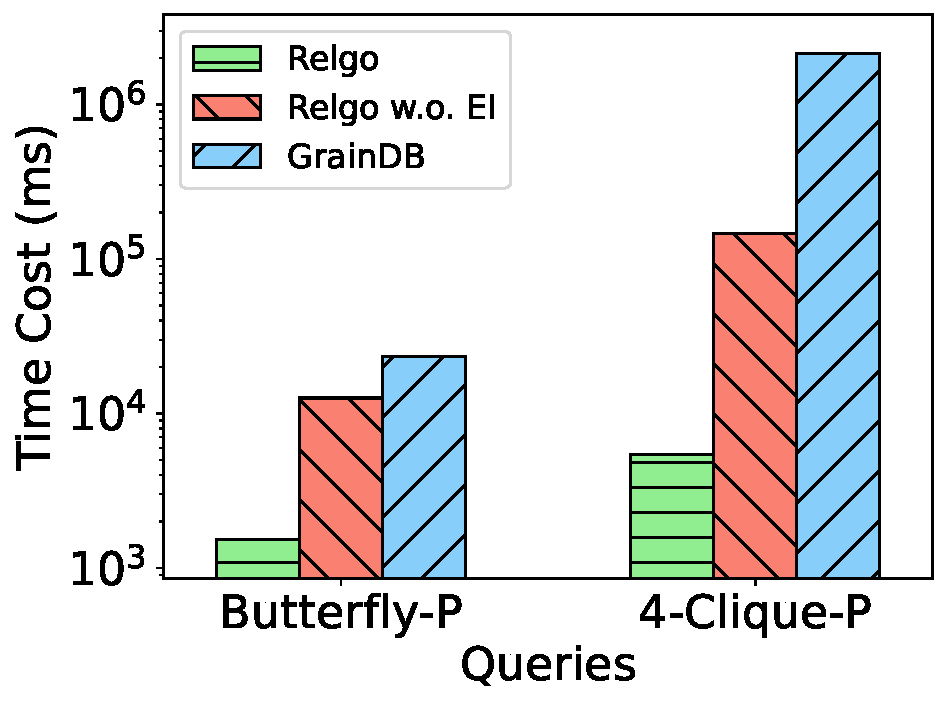
\includegraphics[width=\linewidth]{./figures/exp/ablation_ei_para_sf10.pdf}
        \caption{Time Cost on $G_{sf10}$.}
        \label{fig:exp-expand-intersect-sf10}
    \end{subfigure}
    \begin{subfigure}[b]{0.45\linewidth}
        \centering
        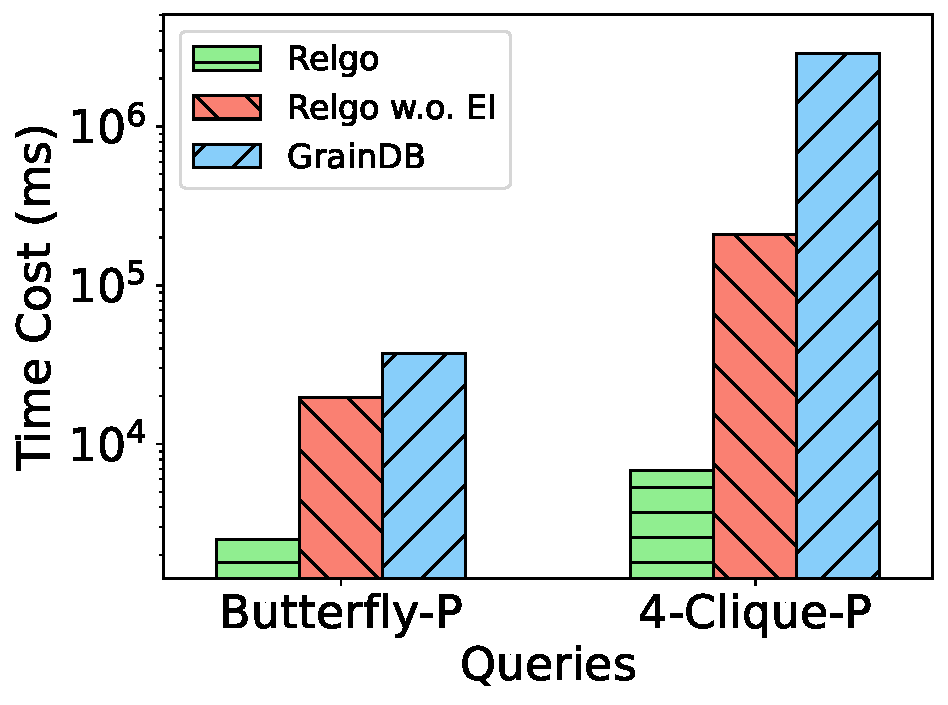
\includegraphics[width=\linewidth]{./figures/exp/ablation_ei_para_sf30.pdf}
        \caption{Time Cost on $G_{sf30}$.}
        \label{fig:exp-expand-intersect-sf30}
    \end{subfigure}
    \caption{Ablation study on \expandintersectrule with constrained-patterns}
    \label{fig:exp-expand-intersect}
\end{figure}

Furthermore, we evaluate the efficiency of \expandintersectrule~ in \relgo. 
In detail, when \expandintersectrule~ is not applied, the extend-intersect operators in the plans are replaced with multiple join operators, and this variant of \relgo is denoted as \textit{\relgo w.o. EI}.
Since \expandintersectrule~ is designed to optimize queries with cycles, we conduct experiments with queries $Q_c[1\ldots 3]$, which consists of patterns with cycles, on $G_{sf10}$ and $G_{sf30}$.
We compare the performance of \relgo and \textit{\relgo w.o. EI} on these queries, and the results are shown in Fig.~\ref{fig:exp-expand-intersect}.
The results suggest that \expandintersectrule~ can significantly enhance the efficiency of \relgo~ on queries with cycles...\todo{wip: analysis}.

% In this section, we conduct ablation study to show the efficiency of \expandintersectrule.
% In detail, patterns in Fig.~\ref{fig:exp-hard-patterns} are queried on $G_{sf10}$ and $G_{sf30}$, and plans are optimized with Relgo.
% For each plan optimized by Relgo, we replace the extend-intersect operators in it with multiple join operators and obtain a new plan.
% These new plans are called obtained with \textit{"Relgo w.o. EI"}.
% The experimental results are shown in Fig.~\ref{fig:exp-ablation-ei}.

% The results illustrate the efficiency of \expandintersectrule.
% When triangles are searched for, removing the extend-intersect operators decreases the query performance.
% Besides, when butterflies and 4-cliques are searched for, the plans without extend-intersect operators have an excessive memory overhead and cause an ``Out of Memory'' (abbr.~OOM) error.
% The reason is that applying extend-intersect operators has much fewer intermediate results than applying multiple joins, since numerous results that will not appear in the intersection are prematurely deleted.
% It indicates that \expandintersectrule can not only enhance query performance, but also reduce spatial overhead.

% To further demonstrate the efficiency of \expandintersectrule, we add predicates on butterflies (i.e., Fig.~\ref{fig:exp-hard-butterfly}) and 4-cliques (i.e., Fig.~\ref{fig:exp-hard-clique}) to avoid OOM, and generate two new patterns, i.e., \textit{Butterfly-P} and \textit{4-Clique-P}. 
% Specifically, for these two new patterns, the values of properties Person1.\textit{p\_personid} are constrained to be smaller than specified values.
% Queries of these new patterns are optimized with GrainDB, \relgo, and \textit{\relgo w.r. EI}.
% The results on the constrained-patterns are shown in Fig.~\ref{fig:exp-ablation-para-ei}.


% The results suggest that \expandintersectrule is crucial in optimizing queries with cycles.
% Specifically, for the new patterns with cycles, the execution time of plans optimized by \relgo is more than an order of magnitude shorter than those optimized by \textit{"Relgo w.o. EI"}.
% It indicates the effectiveness of \expandintersectrule.
% Moreover, when patterns with many cycles are used (e.g., 4-clique in Fig.~\ref{fig:exp-hard-clique}), the optimization effect of the rule becomes particularly noticeable.
% In detail, querying for 4-cliques with \relgo can be 100$\times$ faster than with \textit{"Relgo w.o. EI"}.
% The results illustrate the efficiency of \expandintersectrule.

\begin{figure*}[ht]
    \centering
    \begin{subfigure}[b]{0.45\linewidth}
        \centering
        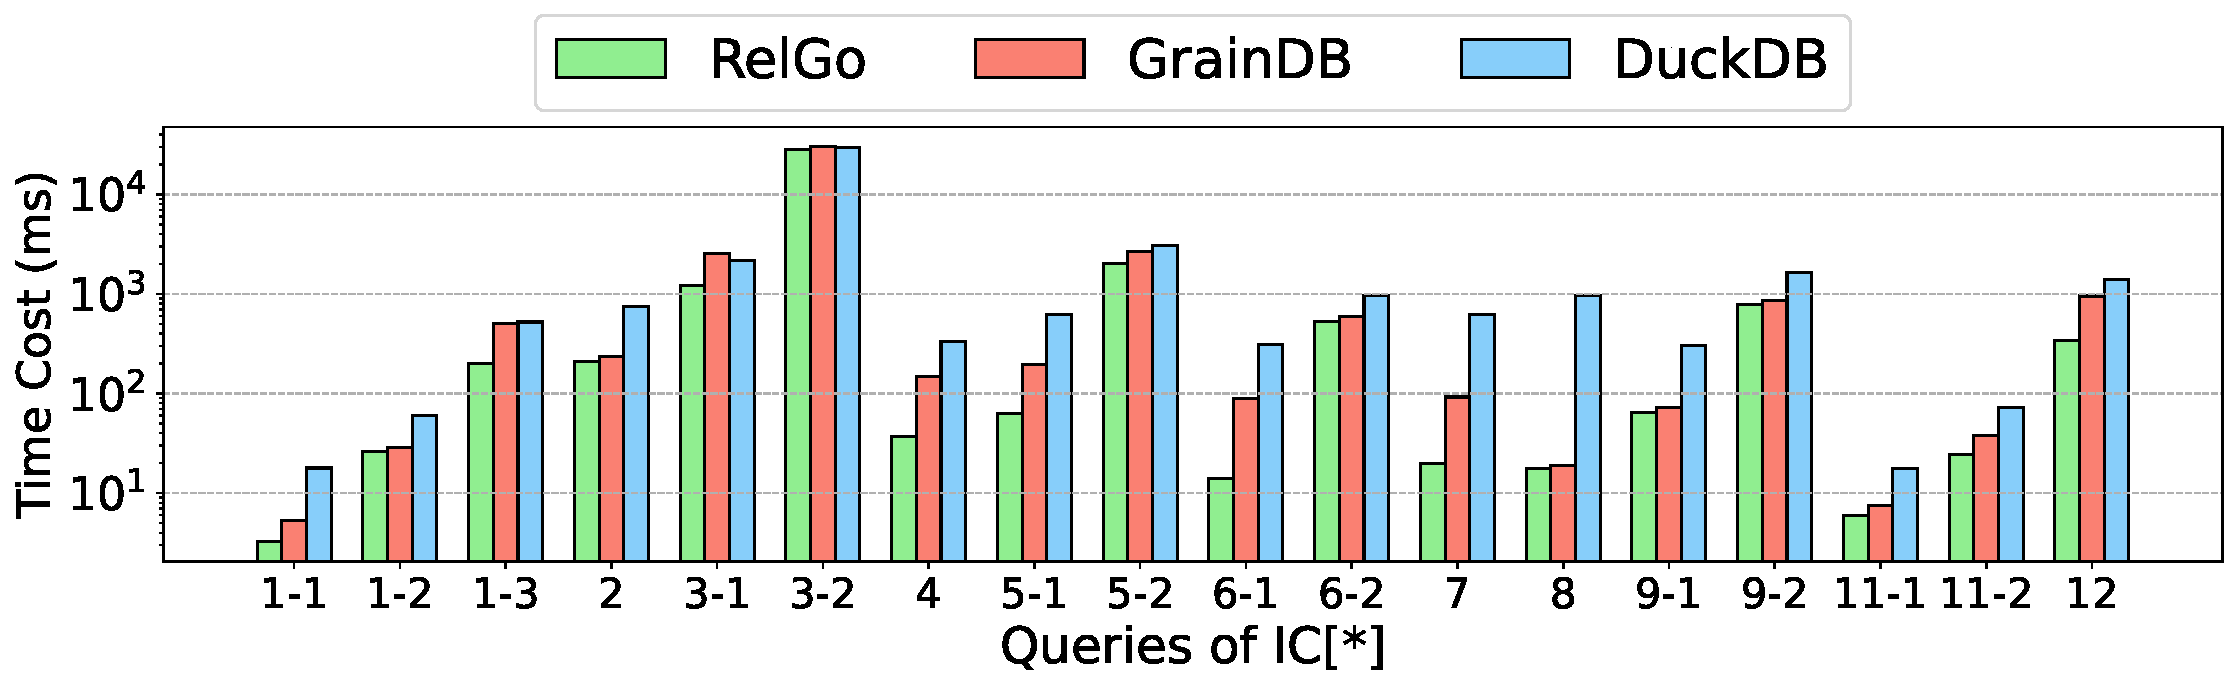
\includegraphics[width=\linewidth]{./figures/exp/e2e_sf10.pdf}
        \caption{Time Cost on $G_{sf10}$.}
        \label{fig:exp-e2e-sf10}
    \end{subfigure}
    \begin{subfigure}[b]{0.45\linewidth}
        \centering
        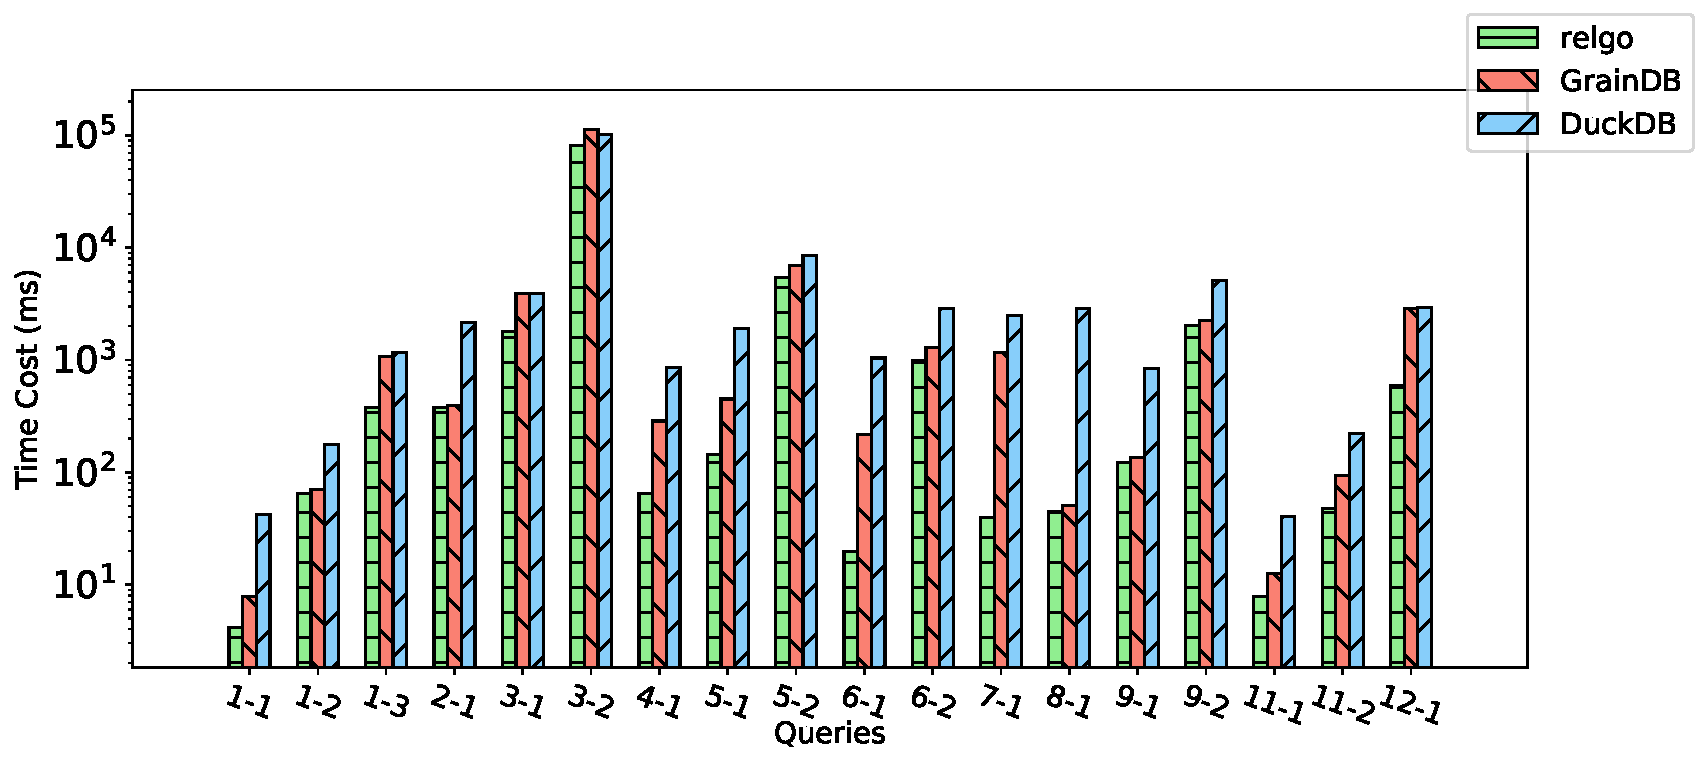
\includegraphics[width=\linewidth]{./figures/exp/e2e_sf30.pdf}
        \caption{Time Cost on $G_{sf30}$.}
        \label{fig:exp-e2e-sf30}
    \end{subfigure}
    \begin{subfigure}[b]{0.6\linewidth}
        \centering
        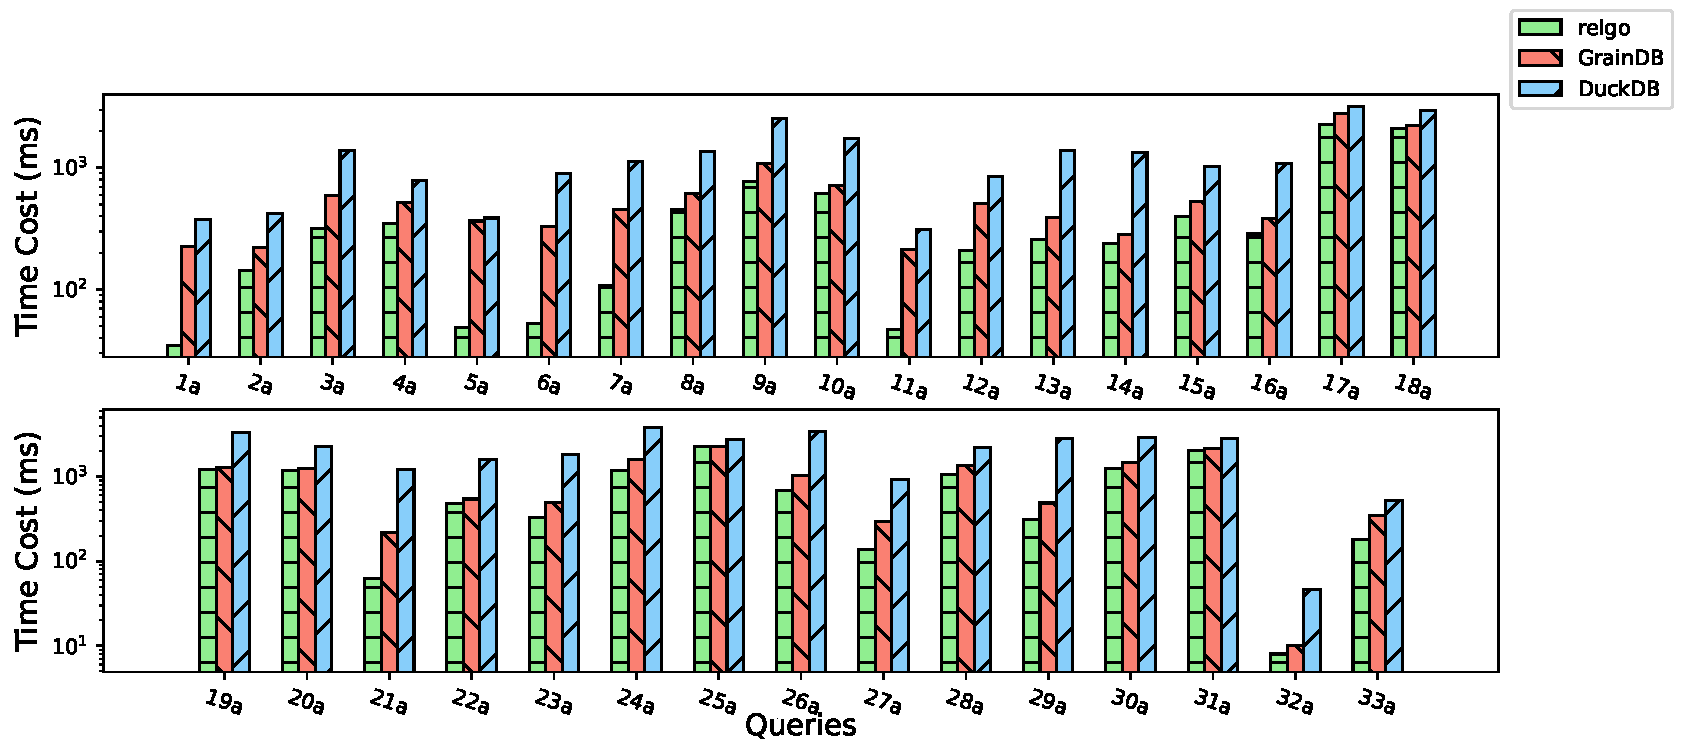
\includegraphics[width=\linewidth]{./figures/exp/e2e_job.pdf}
        \caption{Time Cost on IMDB.}
        \label{fig:exp-e2e-job}
    \end{subfigure}
    \caption{Results of the end-to-end experiments.}
    \label{fig:exp-e2e}
\end{figure*}

\subsection{End-to-End Experiments}
\label{sec:experiment-e2e}

End-to-end experiments are conducted on SNB-M and JOB benchmarks to compare the performances of execution plans obtained by DuckDB, GrainDB, and \relgo.
For experiments on the LDBC benchmark, each IC query is executed for 50 times with different times, and the average time cost is reported.
The experimental results are shown in Fig.~\ref{fig:exp-e2e}.

The results demonstrate that the execution plans obtained with \relgo are always better than those obtained with GrainDB and DuckDB.
For example, when query 1a is queried on the IMDB dataset, executing the plan from \relgo is about 6$\times$ and 10$\times$ faster than executing the plans from GrainDB and DuckDB, respectively.
There are mainly two reasons for the superiority of \relgo.
Firstly, \relgo is aware of the existence of graph indices in graph query optimization.
Thus, the cost estimation of \relgo is more accurate and better physical plans can be obtained.
In contrast, the optimizers of DuckDB and GrainDB are of the types $Rel$ and $Rel^+$, respectively, and are not aware of the graph indices in query optimization.
Therefore, the accuracy of cost estimation is limited.
Secondly, for queries with cycles (e.g., IC7-1 on SNB-M), \relgo can replace multiple joins with extend-intersection.
Such an operator can significantly reduce the time consumption, which is demonstrated through experiments in Sec.~\ref{sec:experiment-circle}.
Thirdly, \relgo is more adept at identifying opportunities to effectively utilize graph indices to get neighbors of vertices, since it optimizes graph queries from the graph perspective.
Conversely, GrainDB occasionally partitions the process into separate stages, first retrieving adjacent edges and subsequently obtaining the corresponding endpoints.